% 4yp.tex - 4th Year project report
% Max Jaderberg 2012

%-------------------------------
% Preamble
%-------------------------------
\documentclass[11pt, onecolumn, a4paper, final]{report} % 11pt font
\renewcommand{\familydefault}{\sfdefault} % sans-serif (Arial) font
\linespread{2} % double line spacing
\usepackage{amssymb,amsmath}
\usepackage[hang,small]{caption} % makes captions look nicer
\usepackage{subfig}
\usepackage{graphicx}
\usepackage[margin=20mm]{geometry}

% for code listings
\usepackage{listings}
\usepackage{color}
\definecolor{dkgreen}{rgb}{0,0.6,0}
\definecolor{gray}{rgb}{0.5,0.5,0.5}
\definecolor{mauve}{rgb}{0.58,0,0.82}
\lstset{frame=single,
  language=Java,
  aboveskip=3mm,
  belowskip=3mm,
  showstringspaces=false,
  columns=flexible,
  basicstyle={\small\ttfamily},
  numbers=none,
  numberstyle=\tiny\color{gray},
  keywordstyle=\color{blue},
  commentstyle=\color{dkgreen},
  stringstyle=\color{mauve},
  breaklines=true,
  breakatwhitespace=true
  tabsize=3
}

\usepackage{hyperref} % for hyperlinks


\title{The Intelligent Image}
\author{Max Jaderberg\\
	Keble College, University of Oxford}
\date{Trinity Term 2012}


%-------------------------------
% Document
%-------------------------------
\begin{document}

\maketitle

\begin{abstract}
In this report, I shall discuss some awesome stuff.
\end{abstract}

%-------------------------------
% Introduction
%-------------------------------
\chapter{Introduction}
The web contains billions of images, which are often the focus of attention on the web pages that include them. However, there is almost no information about the content of these images. Images on websites are purely binary data files, occasionally with some associated meta data included in the image's HTML\footnote{Hyper Text Markup Language \url{http://en.wikipedia.org/wiki/HTML}} code. Very little information is available about the image, let alone the objects or scenes contained within the image. The aim of this project is to create a system which automatically recognises the objects within these images, thus releasing the information within them. This is a large scale object retrieval problem.

There are a large number of applications which would benefit from having detailed information on the contents of images. With more knowledge on the objects contained within images, one can create more effective search engines, better cataloguing and classification systems, user interfaces which engage viewers more, and relevant advertising based on the content. Novel applications could also be built, for example, which retrospectively embed geographical information in the image binary by recognising where the image was photographed. The plethora of useful applications provides a great deal of motivation for this project.

\begin{figure}[ht]
\centering 
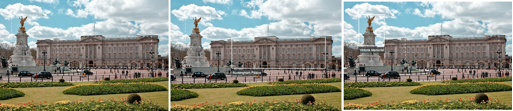
\includegraphics{images/intimage.png}
\caption{An example ``Intelligent Image'' showing the various hover over states}
\label{fig:intimage}
\end{figure}

The result of the project is that a query image is inputted, the objects contained within the image are recognised, and the image is returned with the recognised objects ``tagged'' i.e. the region of the object in the image is outlined and it can be clicked to give relevant information. In this way the standard image has been transformed into the ``intelligent image'' - one which knows about the contained scene and can offer up information to the consumer about it's contents.

Recognising a wide range of objects in an image is not a trivial problem. For such a system to be useful the following needed to be addressed:
\begin{itemize}
\item Acquire and filter enough data to create a model to perform matching on a large range of objects.
\item Create a retrieval system which provides accurate matching. False positive matching needs to be avoided as much as possible.
\item Ensure matching can be done quickly on a database of millions of objects.
\end{itemize}

To recognise millions of different objects, reference images are needed to create a model to match against. From the outset, Wikipedia\footnote{\url{http://en.wikipedia.org}} is used as the primary model data source. Wikipedia is a crowd-sourced online encyclopaedia with many images contained within the articles, and is considered an accurate source of information. In the system, each Wikipedia page defines an object, with the images in the article being used to provide the data to match against. The content of the Wikipedia article is used to give the user further information about the object. A web crawler was written to extract the relevant images of desired Wikipedia pages and create the image database. Filtering is also performed to ensure only useful images are included in the database. The data sources are fully explained in Chapter~\ref{chpt:data}.

Object retrieval uses a method employing a bag-of-words model. This builds upon the work described in x and y, more information of which is provided in Chapter~\ref{chpt:background}. The visual words in the image database from Wikipedia are precomputed. At run time, the words in the query image are computed and searched against the database of precomputed words to find the top image matches. The top matches are spatially verified, with the first verified image being the result. Subsequent improvements to the base line system (described fully in Chapter~\ref{chpt:system}) were made, including geometric improvements to the spatial verification and descriptors used to increase speed and accuracy of spatial verification, and matching improvements through query expansion using crowd-sourced data (dubbed ``Turbo-boosting'') from Microsoft's Bing\footnote{\url{http://www.bing.com}} search engine. The geometric improvements and turbo-boosting is reported in Chapter~\ref{chpt:geoimprovements} and Chapter~\ref{chpt:turboboosting} respectively.

Finally a website was developed to provide a front end interface for the system. A user can simply navigate to the website and upload an image. They then start the automatic tagging process, during which a realtime log of the process is displayed. After the query is complete, the intelligent image is displayed, which the user can interact with, see the names of the objects contained within the image, and click on the object to go to it's Wikipedia page. The software architecture of the website and the backend systems is explored in Chapter~\ref{chpt:architecture}. The result is a realtime automatic tagging system which could recognise, for example, all the buildings in a tourist's photo album of London in seconds.

The aim of the project is to work towards recognising every object on Wikipedia, however due to time restraints a subset of objects was used for development and testing of the project. The subset chosen were the pages that appear on the Wikipedia page ``List of Structures in London''\footnote{\url{http://en.wikipedia.org/wiki/List_of_structures_in_London}}.
	

%-------------------------------
% Background
%-------------------------------
\chapter{Background}
\label{chpt:background}


%-------------------------------
% Data
%-------------------------------
\chapter{Data}
\label{chpt:data}
There are three main datasets used by the application: the images from Wikipedia used to build the database of objects (Section~\ref{sec:modelimages}), the images from Microsoft Bing used for the Turbo-boosting (Section~\ref{sec:turboimages}) and the images from Google Images used for validation and testing (Section~\ref{sec:validationimages}). All images that are used are resized so that their larger dimension does not exceed 1000 pixels to reduce storage space and provide homogeneity. This chapter describes the various datasets and how they are acquired. Table~\ref{tbl:data} gives an overview of the data used.

\begin{table}[hbtp]
\begin{center}
\begin{tabular}{c|c|c|c|}
\cline{2-4}
 & Source &  \# Images &  \# Classes \\ 
 \cline{1-4}
\multicolumn{1}{|c|}{Model images} & Wikipedia & \texttt{3963} & \texttt{732} \\  
\cline{1-4}
\multicolumn{1}{|c|}{Turbo-boosting images} & Microsoft Bing & \texttt{18273} & \texttt{732} \\  
\cline{1-4}
\multicolumn{1}{|c|}{Validation images} & Google &  \texttt{701} & \texttt{294} \\  
\cline{1-4}
\end{tabular}
\end{center}
\caption{A summary of the datasets.}
\label{tbl:data}
\end{table}

\section{Model Images}
\label{sec:modelimages}
The model comprises of a dataset of images that depict the objects that are to be able to be recognised. 

Each page of Wikipedia that contains images represents an object which can be matched. The database of images which is used to build the model is simply created by visiting each page on Wikipedia for the objects desired and downloading the relevant images contained on the web page, labelling those images as being associated with the object. A script automates this process of building the model database.

\begin{figure}[htb]
\centering 
\subfloat[]{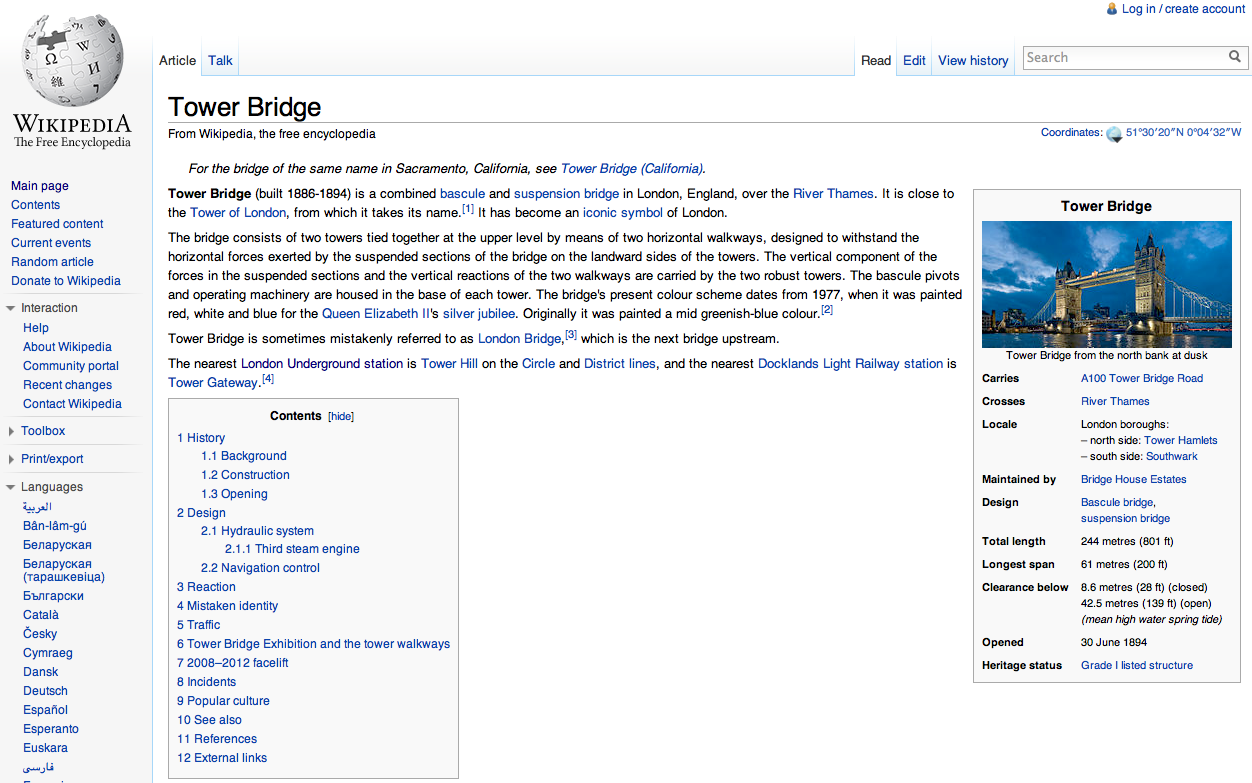
\includegraphics[width=0.5\textwidth]{images/wikipedia-article1.png}}
\subfloat[]{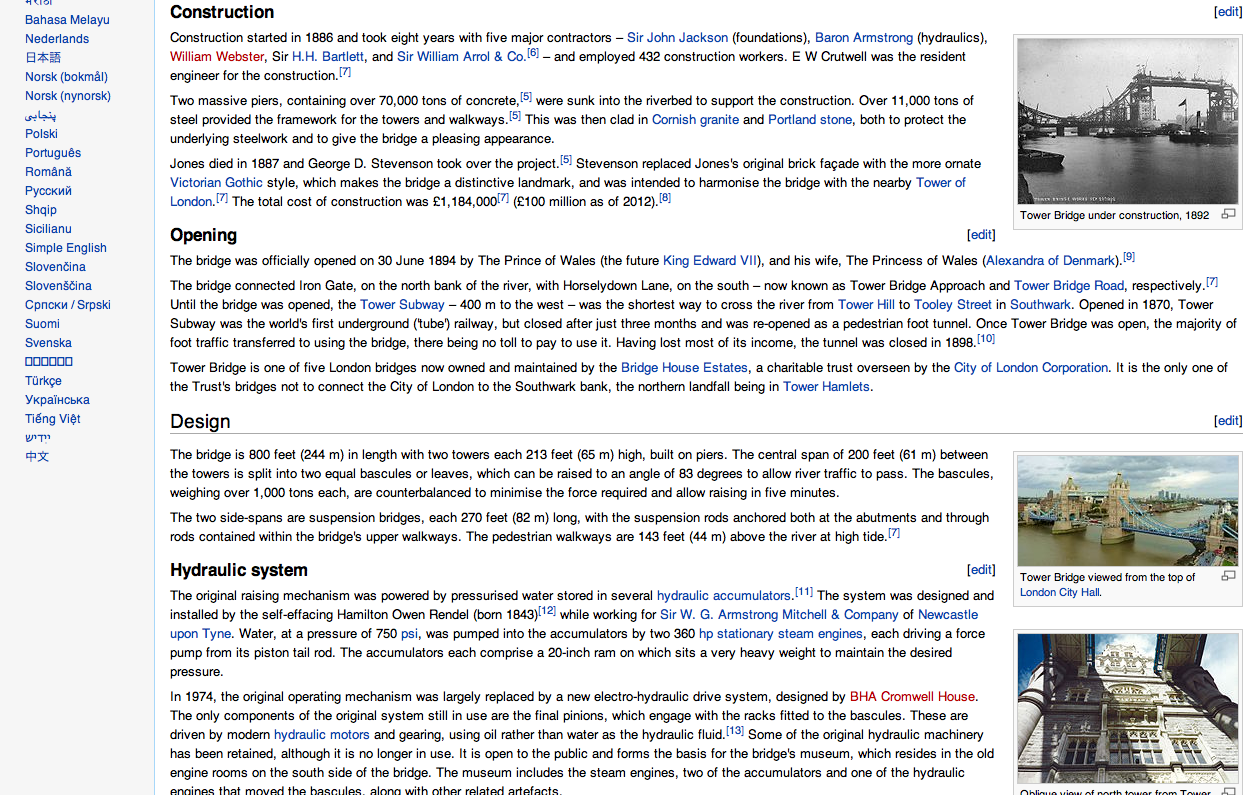
\includegraphics[width=0.5\textwidth]{images/wikipedia-article2.png}}
\caption{The Wikipedia page for ``Tower Bridge''. Note the images contained are those used in the model to represent this object.}
\label{fig:wikipage}
\end{figure}

To automate the downloading of object images from Wikipedia, Python\footnote{\url{http://www.python.org}} is used. WIkipedia offers a public application programming interface (API) over HTTP to access its data, as it is built on the MediaWiki framework\footnote{The MediaWiki framework was originally developed for Wikipedia and provides an API over HTTP as standard. \url{http://www.mediawiki.org/wiki/API} provides documentation for the API.}. However it is cumbersome and not easy to consume. Instead, a web crawler was written to explore Wikipedia pages and extract the relevant images. 

A crawler object in Python finds all the images and notes the URLs of them for subsequent download. Firstly, the HTML of the Wikipedia page must be downloaded, as it appears to a web browser (an example of a web browser being Google Chrome). However, Wikipedia does not allow crawlers and automated bots to access its web pages. To overcome this, the HTTP header\footnote{\url{http://www.w3.org/Protocols/rfc2616/rfc2616.html} describes the Hyper Text Transport Protocol and the various header fields.} of the crawler is edited to emulate that of a browser. This is implemented using the urllib2 library\footnote{\url{http://docs.python.org/library/urllib2.html}}. The code shown in Listing~\ref{lst:crawler} shows an example of how to read the HTML of the main Wikipedia homepage. The HTML document for each Wikipedia page is parsed using the BeautifulSoup library\footnote{\url{http://www.crummy.com/software/BeautifulSoup/}}. All the anchor elements are found and stored for further crawling. The images contained within the HTML are also found by looking within the part of the HTML document that is unique to the specific Wikipedia page (see Listing~\ref{lst:beautifulsoup}).

\linespread{1} % single line spacing
\lstset{language=Python,caption=The code used to gain access to Wikipedia's content using a crawler by emulating a browser.,label=lst:crawler}
\begin{lstlisting}[frame=single]
## Python
import urllib2
# Emulate the user agent as that of a browser
user_agent = "Mozilla/5.0 (Macintosh; U; Intel Mac OS X; en-US; rv:1.8.1.7) Gecko/2007091417 Firefox/2.0.0.7"
headers = {"User-Agent": user_agent}
# Request the webpage
req = urllib2.Request("http://en.wikipedia.org", headers=headers)
resp=urllib2.urlopen(req)
# Read the HTML of the response
html = resp.read()
\end{lstlisting}
\linespread{2} % double line spacing



\linespread{1} % single line spacing
\lstset{language=Python,caption=Parsing the Wikipedia article HTML document to find the relevent images.,label=lst:beautifulsoup}
\begin{lstlisting}[frame=single]
## Python
def _get_content_body(self, soup):
        main_content = soup.find('div', {"class": "mw-content-ltr"})
        if main_content is None:
            return None
        # remove navboxes
        navboxes = main_content.findAll('table', {'class': 'navbox'})
        [navbox.extract() for navbox in navboxes]
        return main_content

def _get_image_links(self, soup):
	return soup.findAll('a', {'class': 'image'})
	
# Parse the HTML
soup = BeautifulSoup(html)
# Get the main article body
soup = _get_content_body(soup)
# Get a list of image links
image_links = _get_image_links(soup)
\end{lstlisting}
\linespread{2} % double line spacing


The output of the crawler is a CSV file of the image URLs and the object class the images belong to. The object class is simply named from the URL of the Wikipedia page (for example all images appearing on \url{http://en.wikipedia.org/wiki/Tower_Bridge} will have class \lstinline!Tower_Bridge!).

The images mentioned in the CSV file produced by the crawler are then downloaded to local storage. Each image that appears on Wikipedia has a ``file page'' which displays the image along with properties and metadata on the image\footnote{For an example see \url{http://en.wikipedia.org/wiki/File:Tower_bridge_London_Twilight_-_November_2006.jpg}}. This ``file page'' is visited for each image, and the page is parsed to extract the storage URL of the image as well as its file format and original size. As the application resizes all images that exceed 1000 pixels to 1000 pixels, it is a waste of time and storage space to download the original image and later resize it. Instead, Wikipedia's inbuilt thumbnail engine is exploited, which resizes the image on Wikipedia's servers and allows you to download a thumbnail of a user selected width\footnote{\url{http://www.algorithm.co.il/blogs/programming/wikipedia-images/} describes how this is exploited}. Therefore if the original image on Wikipedia exceeds 1000 pixels, the 1000 pixel thumbnail version is downloaded instead. The images downloaded are saved in a folder named after it's class. The result is a directory containing a folder for each class, within which are the images for that class.

This process creates a structured dataset of model images from the Wikipedia pages visited. For the List of Structures in London dataset used, there were 732 classes which had 3963 images associated with them (on average 6 images per class).


\section{Turbo-boosting Images}
\label{sec:turboimages}
To achieve effective turbo-boosting, many additional images are needed to supplement the model images acquired from Wikipedia. Microsoft Bing is used as the source of the turbo-boosting images. For each class, 25 additional images are downloaded to boost that class.

Bing offers a public API that can be used to perform image searches programmatically. After obtaining an application ID from Bing for authentication, complex search requests can be made over HTTP, with the results returned in JavaScript Object Notation (JSON) format\footnote{JSON is an alternative to XML for representing structured data. \url{http://www.json.org/} provides more information.}.

Bing image search takes a number of keywords - the query - and returns a list of images from web pages related to the query. Further filters can be applied to further narrow down the search to the most relevant images. This is shown in Figure~\ref{fig:bingimages} on the website version of Bing. The ``Style'' and ``Size'' filters are especially useful in this application, as all images should be photographs for the List of Structures in London dataset, and large images are preferable so as to include as much detail as possible. Setting these filters precludes many instances of graphics and logos which are not suitable for turbo-boosting.

\begin{figure}[htb]
\centering 
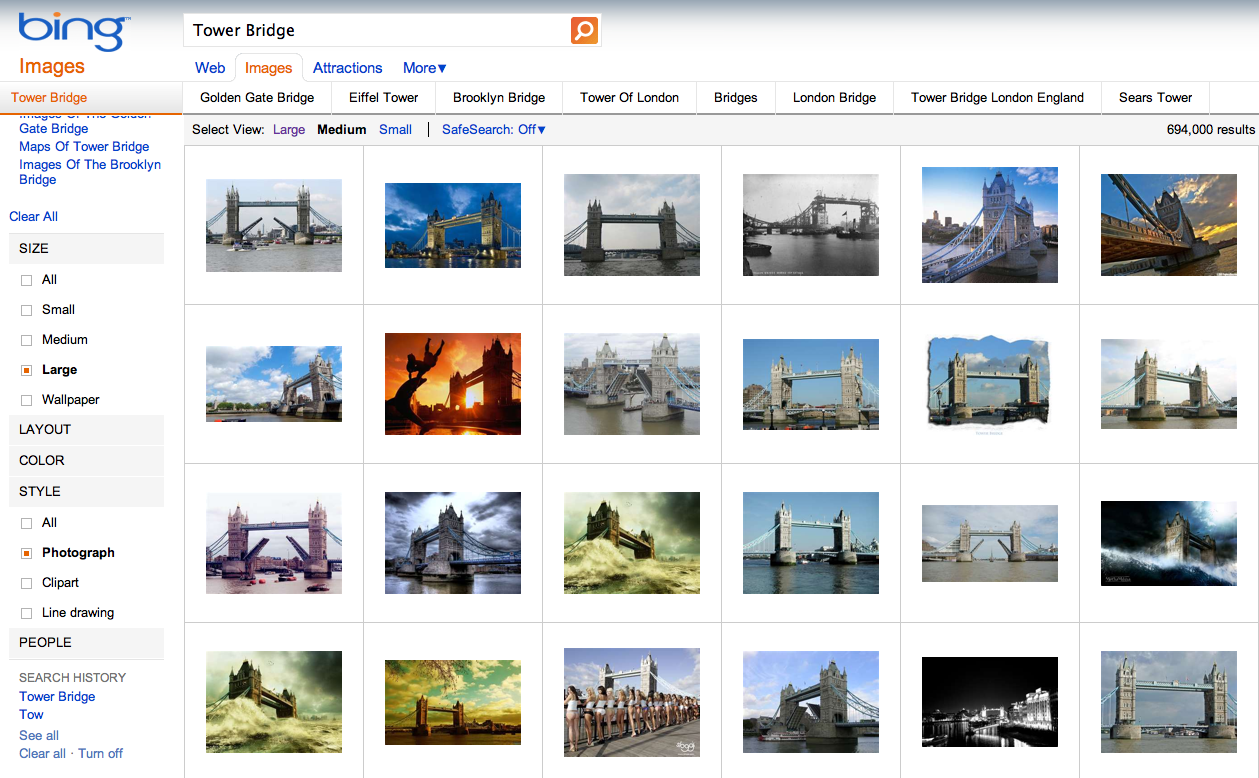
\includegraphics[width=0.9\textwidth]{images/bing-images.png}
\caption{The browser interface of Bing image search which is replicated in the API query URL. Note the filters in the left column.}
\label{fig:bingimages}
\end{figure}

All the parameters that appear in the web interface for Bing image search can be replicated in the API request with query parameters. A MATLAB script is used to consume the API and download the images. Listing~\ref{lst:bingapi} shows the URL used for the API call to get the search results for the images for a particular class. The URL encoded\footnote{URL encoding ensures that all characters are in a form which can be used as a URL. See \url{http://www.w3schools.com/tags/ref_urlencode.asp} for more information.} class name is used as the query. For example, for the class \lstinline!Tower_Bridge!, the variable \lstinline!search_term! appearing in Listing~\ref{lst:bingapi} will be set to \lstinline!"Tower%20Bridge"! (note \lstinline{" "} is URL encoded as \lstinline{"%20"}). Both the ``Style'' and ``Size'' image filters are set to ``Photo'' and ``Large'' respectively by setting the \lstinline!Image.Filters! parameter.

\linespread{1} % single line spacing
\lstset{language=Matlab,caption=A Bing image search API request.,label=lst:bingapi}
\begin{lstlisting}[frame=single]
%% MATLAB
request_url = ['http://api.bing.net/json.aspx?' ...
                   'AppId=' app_id ...
                   '&Query=' search_term ...
                   '&Sources=Image' ...
                   '&Version=2.0' ...
                   '&Adult=Strict' ...
                   '&Image.Count=' nPhotos ...
                   '&Image.Filters=Style:Photo+Size:Large' ...
                   '&JsonType=raw' ...
                  ];
% Read the result of the request
response = urlread(request_url);
% Parse the result from JSON to MATLAB structure form
resp_struct = parse_json(response);
\end{lstlisting}
\linespread{2} % double line spacing

Using MATLAB's inbuilt \lstinline!urlread! function, the search results are requested and returned in JSON format. The JSON result is then parsed and converted into a MATLAB structure object for reading. An example JSON response is shown in Listing~\ref{lst:bingjson}. Each element in the array \lstinline!Results! is an image result. Each image is then downloaded from its \lstinline!MediaUrl! field using a modified version of the \lstinline!imread! function which allows for request timeouts, as some image resources may have expired since their submission to the Bing database.

\linespread{1} % single line spacing
\lstset{language=Java,caption=A Bing image search response in JSON format. The ``Results'' array is truncated to one element.,label=lst:bingjson}
\begin{lstlisting}[frame=single]
// JSON
{
   "SearchResponse":{
      "Version":"2.0",
      "Query":{
         "SearchTerms":"Tower Bridge"
      },
      "Image":{
         "Total":780000,
         "Offset":0,
         "Results":[
            {
               "Title":"Tower Bridge - London Photo (551176) - Fanpop",
               "MediaUrl":"http://images.fanpop.com/images/image_uploads/Tower-Bridge.jpg",
               "Url":"http://www.fanpop.com/spots/london/images/551176/title/tower-bridge",
               "DisplayUrl":"http://www.fanpop.com/spots/london/images/title/tower-bridge",
               "Width":1600,
               "Height":1200,
               "FileSize":761104,
               "Thumbnail":{
                  "Url":"http://ts3.mm.bing.net/images/thumbnail.aspx?q=4757...",
                  "ContentType":"image/jpeg",
                  "Width":160,
                  "Height":120,
                  "FileSize":3274
               }
            }, ...
         ]
      }
   }
}
\end{lstlisting}
\linespread{2} % double line spacing

The downloaded images are resized if larger than 1000 pixels and stored in a folder named after its class. As for the model images, the result is a directory containing a folder for each class, within which are the turbo-boosting images for that class.

\section{Validation Images}
\label{sec:validationimages}

Images are needed to test and validate the yield performance of the object recognition system. Therefore a separate dataset of images with their ground truth classes is needed. Ideally all classes would be tested and each test image should be a fair representation of the object of that class. Google image search was used first to automatically download 8 images for each class. The images were then checked manually to refine the dataset.

Google image search is very similar to Bing image search described in the previous section. However the results are markedly different, providing another set of images that are perfect for testing. Google offers an API over HTTP which can be used to search based on a text query and, as with Bing, filters can be applied. The result is returned in JSON format.

\linespread{1} % single line spacing
\lstset{language=Matlab,caption=A Google image search API request.,label=lst:googleapi}
\begin{lstlisting}[frame=single]
%% MATLAB
request_url = ['https://ajax.googleapis.com/ajax/services/search/images?v=1.0' ...
	'&q=' search_term ...
	'&as_filetype=jpg' ...
	'&imgsz=xxlarge' ...
	'&imgtype=photo' ...
	'&rsz=8' ...
];
% Read the result of the request
response = urlread(request_url);
% Parse the result from JSON to MATLAB structure form
resp_struct = parse_json(response);
\end{lstlisting}
\linespread{2} % double line spacing

Listing~\ref{lst:googleapi} shows the formulation and request of a Google search API request. As with the Bing requests, the search term is the URL encoded class name. The JSON response (Listing~\ref{lst:googlejson}) is parsed into a MATLAB object and the \lstinline!url! field is used to download the image.

\linespread{1} % single line spacing
\lstset{language=Java,caption=A Google image search response in JSON format. The ``results'' array is truncated to one element.,label=lst:googlejson}
\begin{lstlisting}[frame=single]
// JSON
{
   "responseData":{
      "results":[
         {
            "GsearchResultClass":"GimageSearch",
            "width":"1024",
            "height":"819",
            "imageId":"ANd9GcSTU9Qv93OE3Q5kjo0h5Dcsl6sYBGURxSlmw8tfUbISx6heecXcY9VKkquZ",
            "tbWidth":"150",
            "tbHeight":"120",
            "unescapedUrl":"http://www2.hiren.info/desktopwallpapers/natural/the-tower-...",
            "url":"http://www2.hiren.info/desktopwallpapers/natural/the-tower-bridge.jpg",
            "visibleUrl":"www.hiren.info",
            "title":"Desktop Wallpapers � Natural Backgrounds � The \u003cb\u003eTower Bridge\u003c/b\u003e \u003cb\u003e...\u003c/b\u003e",
            "titleNoFormatting":"Desktop Wallpapers � Natural Backgrounds � The Tower Bridge ...",
            "originalContextUrl":"http://www.hiren.info/desktop-wallpapers/natural-pic...",
            "content":"The \u003cb\u003eTower Bridge\u003c/b\u003e, London,",
            "contentNoFormatting":"The Tower Bridge, London,",
            "tbUrl":"http://t1.gstatic.com/images?q\u003dtbn:ANd9GcSTU9Qv93OE3Q5kjo..."
         }, ...
      ], ...
   "responseDetails":null,
   "responseStatus":200
}
\end{lstlisting}
\linespread{2} % double line spacing

As with the turbo-boosting images, the downloaded images are resized if larger than 1000 pixels stored in a folder named after its class. Again, the result is a directory containing a folder for each class, within which are the turbo-boosting images for that class.

After automatic download of potential test images for each class, the dataset was checked over manually. Images that appear in the model dataset, as well as images that do not fairly depict the class they are to test are removed from the test set . 

%-------------------------------
% Base line system
%-------------------------------
\chapter{Base line system}
\label{chpt:system}

%-------------------------------
% Software architecture
%-------------------------------
\chapter{Software architecture}
\label{chpt:architecture}


%-------------------------------
% Geometric Improvements
%-------------------------------
\chapter{Geometric Improvements}
\label{chpt:geoimprovements}


%-------------------------------
% Turbo-boosting
%-------------------------------
\chapter{Turbo-boosting}
\label{chpt:turboboosting}


%-------------------------------
% Summary
%-------------------------------
\chapter{Summary}


%-------------------------------
% References
%-------------------------------
\begin{thebibliography}{99}

	\bibitem{turcot09}
		P. Turcot and D. G. Lowe.
		Better matching with fewer features: The selection of useful features in large database recognition problems
		In \emph{WS-LAVD, ICCV}, 2009.
	  
\end{thebibliography}

\end{document}